\chapter{Overview of Lightweight Neural Network Architectures and Vegetation Indices for Plant Disease Detection}%
\label{app:annexA}

% \begin{center}
%     \begin{verbatim}
%    annex a 
%     \end{verbatim}
% \end{center}


\section{Lightweight Neural Network Architectures}
Lightweight neural network architectures are designed to be efficient, enabling high performance on resource-constrained devices like mobile phones and edge devices. These models balance accuracy and computational efficiency, making them ideal for real-time applications. The following are some key lightweight architectures and how they address these challenges.


\subsection{MobileNetV1}
MobileNet V1 is a lightweight convolutional neural network that efficiently processes input images by utilizing depthwise separable convolutions to reduce computational cost and model size. Starting with an input image resized to 224×224×3, the network first applies a standard convolution followed by a series of depthwise separable convolutions that decompose standard convolutions into two steps: a depthwise convolution that filters each input channel independently and a pointwise (1×1) convolution that combines these filtered outputs. This approach drastically reduces the number of parameters and operations, as seen in the progressive reduction of feature map dimensions from 112×112×32 to 56×56×64, 28×28×256, and eventually to 7×7×1024 (Figure~\ref{fig:MobileNet}). An average pooling operation then reduces the spatial dimension to 1×1×1024, after which a fully connected layer performs the final classification \parencite{kadam2022efficient}.

\begin{figure}[H] % 'H' needs \usepackage{float}
    \centering
    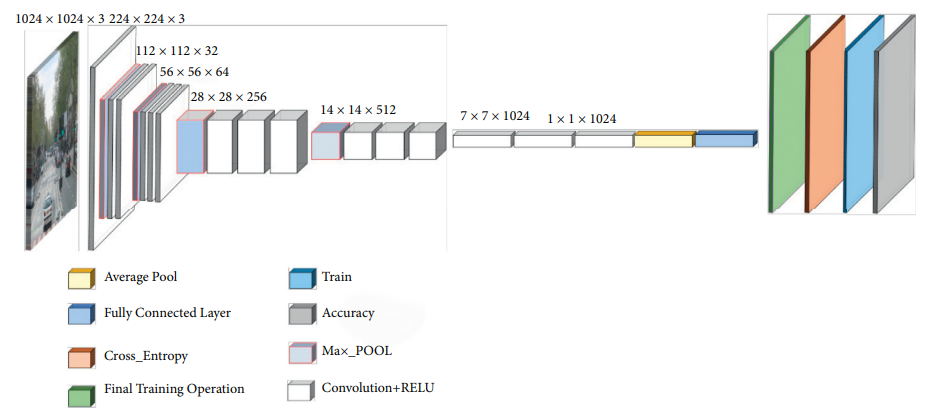
\includegraphics[width=0.8\textwidth]{appendices/images/MobileNet.png}
    \caption{The architecture of MobileNet V1 \parencite{kadam2022efficient}.}
    \label{fig:MobileNet}
\end{figure}


\subsection{EfficientNet}
EfficientNet is a family of convolutional neural networks developed by Google AI that introduces a compound scaling method to efficiently scale deep learning models. Traditional approaches often scale models arbitrarily in one of three dimensions: depth (number of layers), width (number of channels), or input resolution. However, EfficientNet proposes a more balanced and systematic strategy, where all three dimensions are scaled simultaneously and proportionally using a fixed set of scaling coefficients. This compound approach maintains model efficiency while significantly boosting accuracy.

The baseline model, EfficientNet-B0 (see Figure~\ref{fig:figure13}), is built using Neural Architecture Search (NAS) to optimize both performance and efficiency. Larger variants (B1 to B7) are derived by uniformly scaling the baseline model using the compound scaling principle. This results in models that achieve state-of-the-art performance on image classification tasks with dramatically fewer parameters and lower computational cost compared to earlier architectures like ResNet or Inception.

\begin{figure}[H] % 'H' needs \usepackage{float}
    \centering
    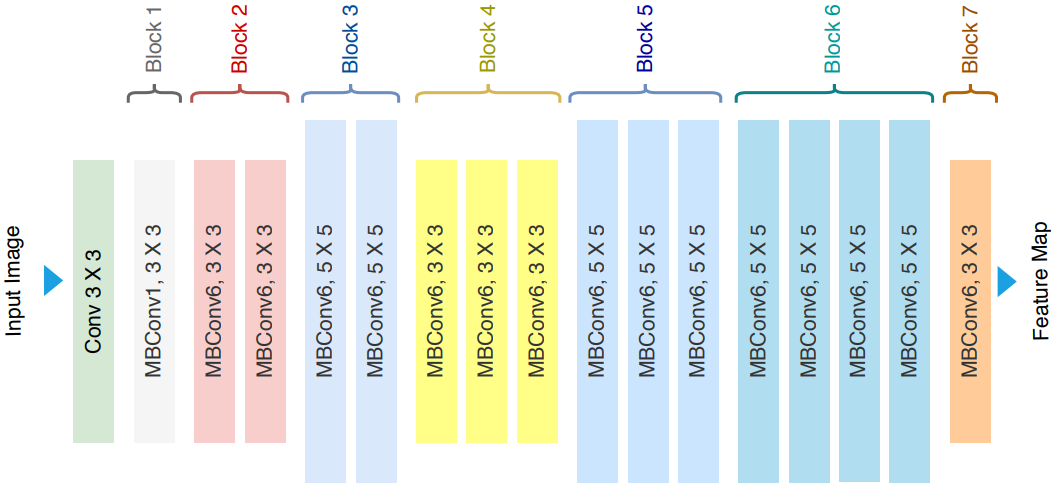
\includegraphics[width=0.8\textwidth]{chapters/chapter1/images/Figure13.png}
    \caption{Architecture of EfficientNet-B0 \parencite{ahmed2022classification}.}
    \label{fig:figure13}
\end{figure}

\subsection{ShuffleNet V2}

ShuffleNet V2 is a family of lightweight convolutional neural networks specifically designed for mobile and embedded platforms with limited computational resources. It improves upon ShuffleNet V1 by addressing practical deployment issues, such as memory access cost and actual inference latency, which are often overlooked in models optimized purely for FLOPs.

Unlike previous versions that relied heavily on group convolutions, ShuffleNet V2 introduces a simpler and more efficient building block. This block incorporates a channel split operation, followed by pointwise and depthwise convolutions, and concludes with a channel shuffle operation. By delaying the channel shuffle to the end of the split-transform-merge sequence, the model enhances feature mixing between channel groups and improves accuracy without incurring a significant computational burden.

These architectural improvements allow ShuffleNet V2 to achieve a strong trade-off between speed and accuracy, making it a highly practical choice for real-time applications in edge computing and mobile vision systems.

\begin{figure}[H]
    \centering
    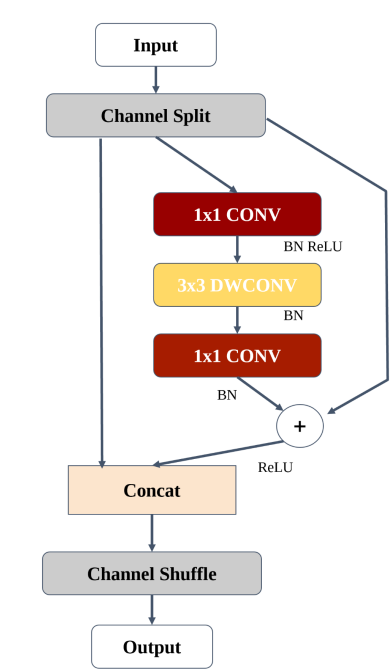
\includegraphics[width=0.4\textwidth]{appendices/images/ShuffleNet.png}
    \caption{\footnotesize Architecture of the basic building block of ShuffleNet V2 with residual connection. CONV: convolution layer; DWCONV: depthwise convolution; BN: batch normalization. Channel Shuffle: a key operation enabling inter-group communication in ShuffleNet architectures \parencite{dobko2020cnn}.}
    \label{fig:ShuffleNet}
\end{figure}


\section{Vegitation Indices}
The table below (Table~\ref{tab:vegetation-indices2}) summarizes the vegetation indices used in the previously discussed studies, along with their formulas and applications.

\begin{table}[htbp]
    \caption{Vegetation Indices and Their Applications (where \( R \) = Red, \( G \) = Green, \( B \) = Blue, and \( NIR \) = Near Infrared)}
    \centering
    \resizebox{\textwidth}{!}{%
    \begin{tabular}{|p{2.5cm}|p{4cm}|p{7.5cm}|p{7cm}|}
    \hline
    \textbf{Reference} & \textbf{Index} & \textbf{Formula} & \textbf{Application} \\
    \hline
    \parencite{bhandari2020assessing} & Green Leaf Index (GLI) & \(\text{GLI} = \frac{2 \times G - R - B}{2 \times G + R + B}\) & Detect green canopy cover in wheat. \\
    \hline
    \parencite{bhandari2020assessing} & Green Index (GI) & \(\text{GI} = \frac{G}{R}\) & Detecting disease stress in crops. \\
    \hline
    \parencite{bhandari2020assessing} & Normalized Difference Index (NDI) & \(\text{NDI} = \frac{G - R}{G + R}\) & Separates plants from soil in RGB images. \\
    \hline
    \parencite{HeidarianDehkordi2020} & Stripe Rust Index (SRI) & \(\text{SRI} = R + G\) & Detects wheat stripe rust infection by identifying yellow-colored regions. \\
    \hline
    \parencite{HeidarianDehkordi2020} & Leaf Rust Index (LRI) & \(\text{LRI} = \frac{2 \times G - R^2}{R \times (G - B)}\) & Identifies wheat leaf rust based on brown color codes by comparing dark and light brown spectral compositions derived from RGB bands. \\
    \hline
    \parencite{guo2021wheat} & SIPI & \(\text{SIPI} = \frac{NIR - B}{NIR - R}\) & Detects carotenoid-to-chlorophyll ratio; useful in early plant stress and senescence monitoring. \\
    \hline
    \parencite{guo2021wheat} & PRI & \(\text{PRI} = \frac{G - B}{G + B}\) & Indicates photosynthetic light use efficiency, sensitive to physiological changes before visible symptoms. \\
    \hline
    \parencite{guo2021wheat} & TCARI & \(\text{TCARI} = 3 \times [(R - G) - 0.2 \times (R - B)] \times \left(\frac{R}{G}\right)\) & Estimates chlorophyll content, compensating for soil background, useful in chlorosis or disease stress. \\
    \hline
    \parencite{guo2021wheat} & PSRI & \(\text{PSRI} = \frac{R - B}{NIR}\) & Indicates leaf senescence and pigment degradation, useful for detecting aging or stressed vegetation. \\
    \hline
    \parencite{guo2021wheat} & YRI & \(\text{YRI} = \frac{NIR - B}{NIR + B - 0.5 \times R}\) & Developed to identify yellow rust in wheat; captures yellowing due to fungal infection. \\
    \hline
    \parencite{guo2021wheat} & MSR & \(\text{MSR} = \frac{\frac{NIR}{R} - 1}{\frac{NIR}{R} + 1}\) & Enhances contrast in vegetation vigor; reduces soil effects; used in disease detection (e.g., powdery mildew). \\
    \hline
    \parencite{guo2021wheat} & MCARI & \(\text{MCARI} = [(G - R) - 0.2 \times (G - B)] \times \left(\frac{G}{R}\right)\) & Highlights chlorophyll absorption, useful in chlorophyll estimation and early stress detection. \\
    \hline
    \parencite{guo2021wheat} & Powdery Mildew Index (PMI) & \(\text{PMI} = \frac{G - R}{G + R - 0.5 \times NIR}\) & Identifies powdery mildew by sensing spectral changes in plant pigments and moisture. \\
    \hline
    \end{tabular}%
    }
    \label{tab:vegetation-indices2}
\end{table}
